\documentclass[12pt,a4paper]{article}
\usepackage[margin=0.75in]{geometry}
\usepackage[utf8]{inputenc}
\usepackage[english]{babel}
\usepackage{amsmath}
\usepackage{amsfonts}
\usepackage{amssymb}
\usepackage{courier}
\usepackage{datetime}
\usepackage{fancyhdr}
\usepackage{float}
\usepackage{graphicx}
\usepackage{lastpage}
\usepackage{makecell}
\usepackage{multicol}
\usepackage{multirow}
\usepackage{pdfpages}
\usepackage{soul}
\usepackage{tabularx}
\usepackage[normalem]{ ulem }
\usepackage{xcolor}
\usepackage{tikz}

\newcommand{\iic}{I\textsuperscript{2}C }
\renewcommand{\familydefault}{\sfdefault}
\renewcommand{\headrulewidth}{0pt}
\renewcommand\theadalign{bc}
\renewcommand\theadfont{\bfseries}
\renewcommand\theadgape{\Gape[4pt]}

\newdateformat{monthyeardate}{%
  \monthname[\THEMONTH], \THEYEAR}

\pagestyle{fancy}
\fancyhf{}
\lhead{Hawkseye - Datasheet}
\lfoot{Frustrating Box}
\cfoot{\thepage / \pageref{LastPage}}
\rfoot{\monthyeardate\today}


\begin{document}

{\raggedleft 
\raisebox{-0.4\height}{
\includegraphics[scale=0.15]{../img/uliege_logo_compact_rvb_pos.pdf}}
}\hfill
%{\raggedright \hspace*{\fill} \huge Hawkseye \hspace*{\fill}}
{\raggedright  \huge Hawkseye}
\begin{center}
 {\huge{Time of flight distance sensor}}\\
 {\large\textit{Based on the VL53L0X from STMicroelectronics}}
\end{center}
\hrulefill
\par\noindent{\large \textbf{Datasheet}}



\section{Introduction}
\begin{multicols}{2}
 This fully open-source sensor is a time-of-flight based distance sensor based on two VL53L0X from STMicroelectronics. It is aimed at providing accurate distance measurements at a high sampling rate which can go up to 50Hz. It is also largely configurable and offers an external interrupt functionality. It accepts a wide input voltage range and will adapt the \iic voltages and interrupt signal to the input power.
 \columnbreak
 \subsection{Features}
 \begin{itemize}
  \item Fully open-source. Adapt it to your needs
  \item Input voltage from 3.0V to 5.5V
  \item Low power consumption
  \item Distance sensing from 0 to 150 cm
  \item \iic communication bus
  \item Programmable \iic address
  \item External interrupts functionality
  \item DIP switches for boot configuration
  \item Embedded calibration routines
 \end{itemize}
\end{multicols}

\subsection{Typical application}

\begin{figure}[h]
 \centering
 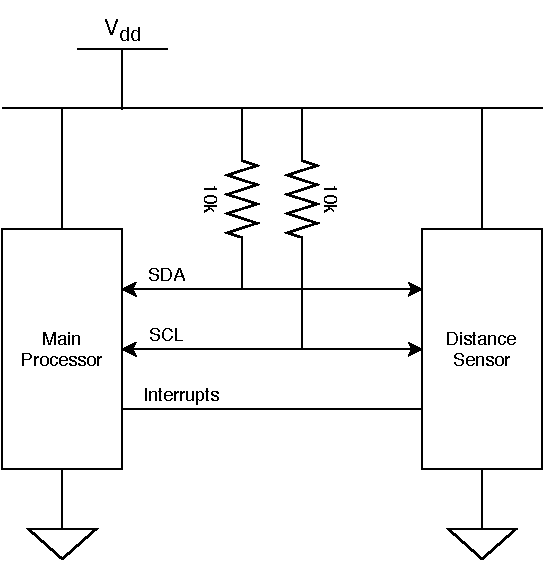
\includegraphics[width=0.5\textwidth]{../img/dual-vl53l0x-sensor.pdf}
\end{figure}
\pagebreak[3]

\section{Layout}
\subsection{Front}
\begin{figure}[h!]
 \centering
 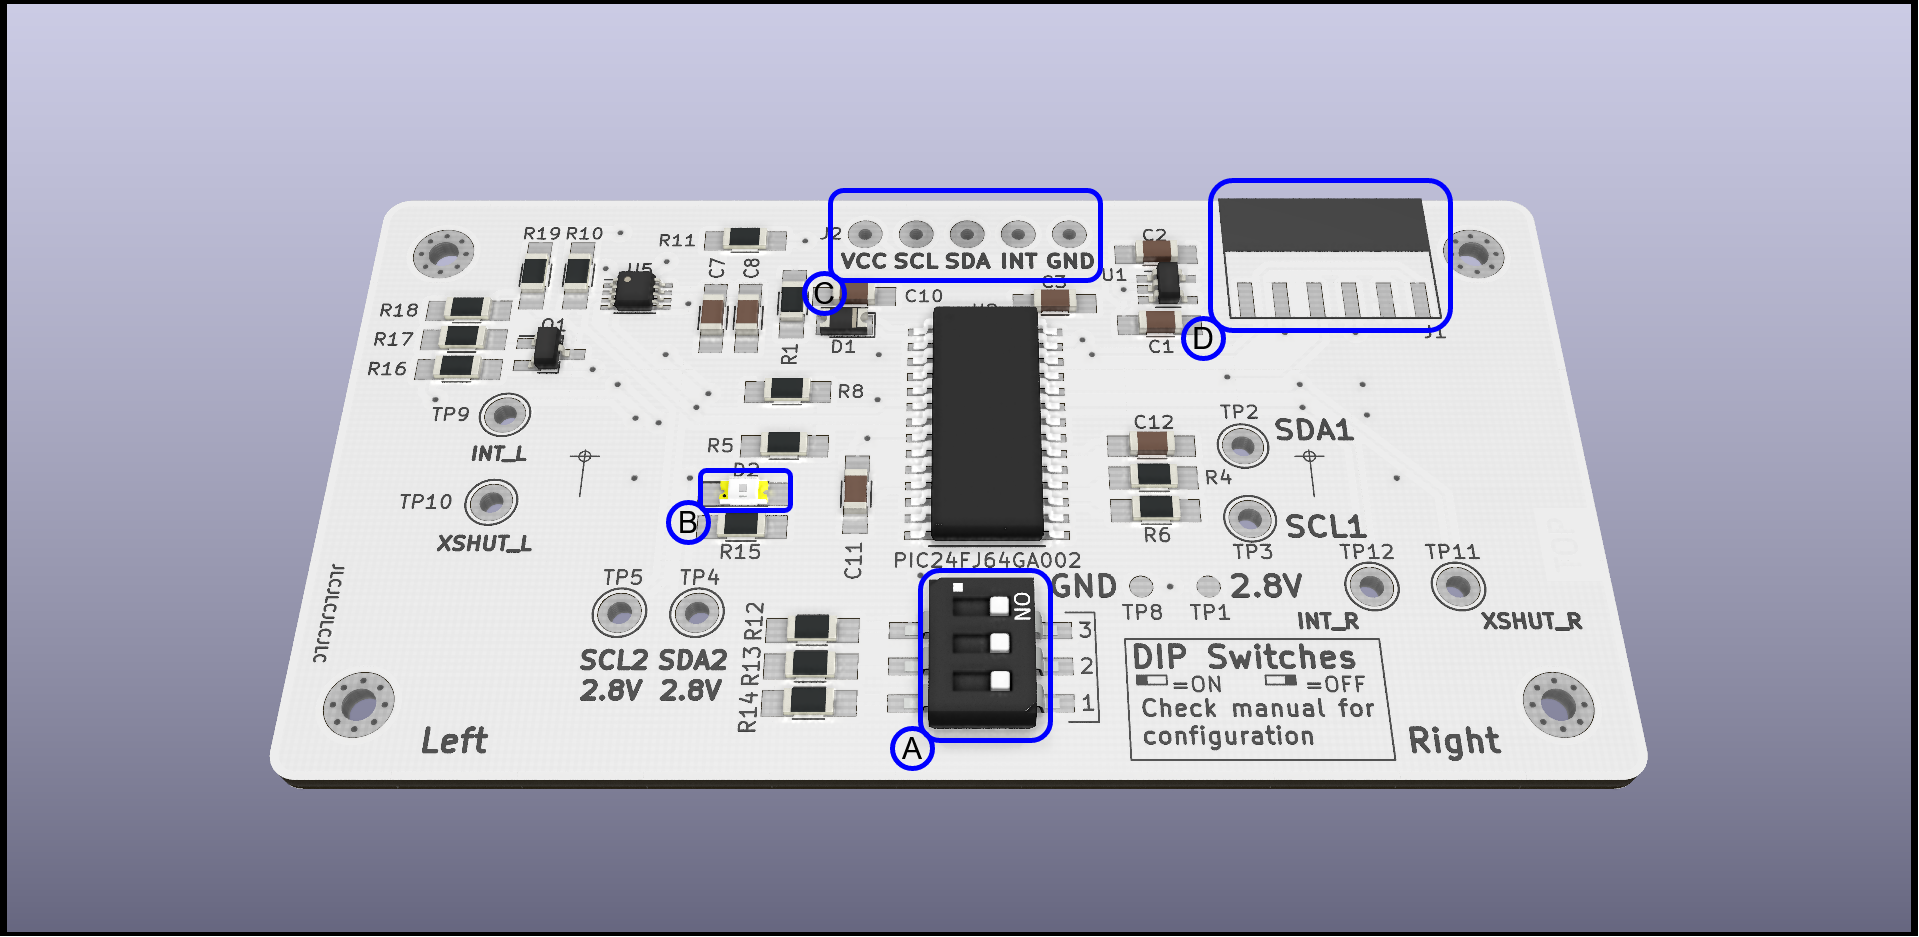
\includegraphics[width=0.75\textwidth]{../img/annotated-layout-front-V1.png}
 \caption{Annotated picture of the front of the sensor}
\end{figure}
\begin{itemize}
 \item[A] Boot configuration DIP Switches.
 \item[B] LED indicator
 \item[C] Main connector (Power, \iic, Interrupts)
 \item[D] ICSP connector to program the PIC controller
\end{itemize}
\textit{\textbf{Note: }On PCB V1.0 the \texttt{XSHUT} and  \texttt{INT} test points labels have been swapped for the right and left sensors.}

\subsection{Back}
\begin{figure}[H]
 \centering
 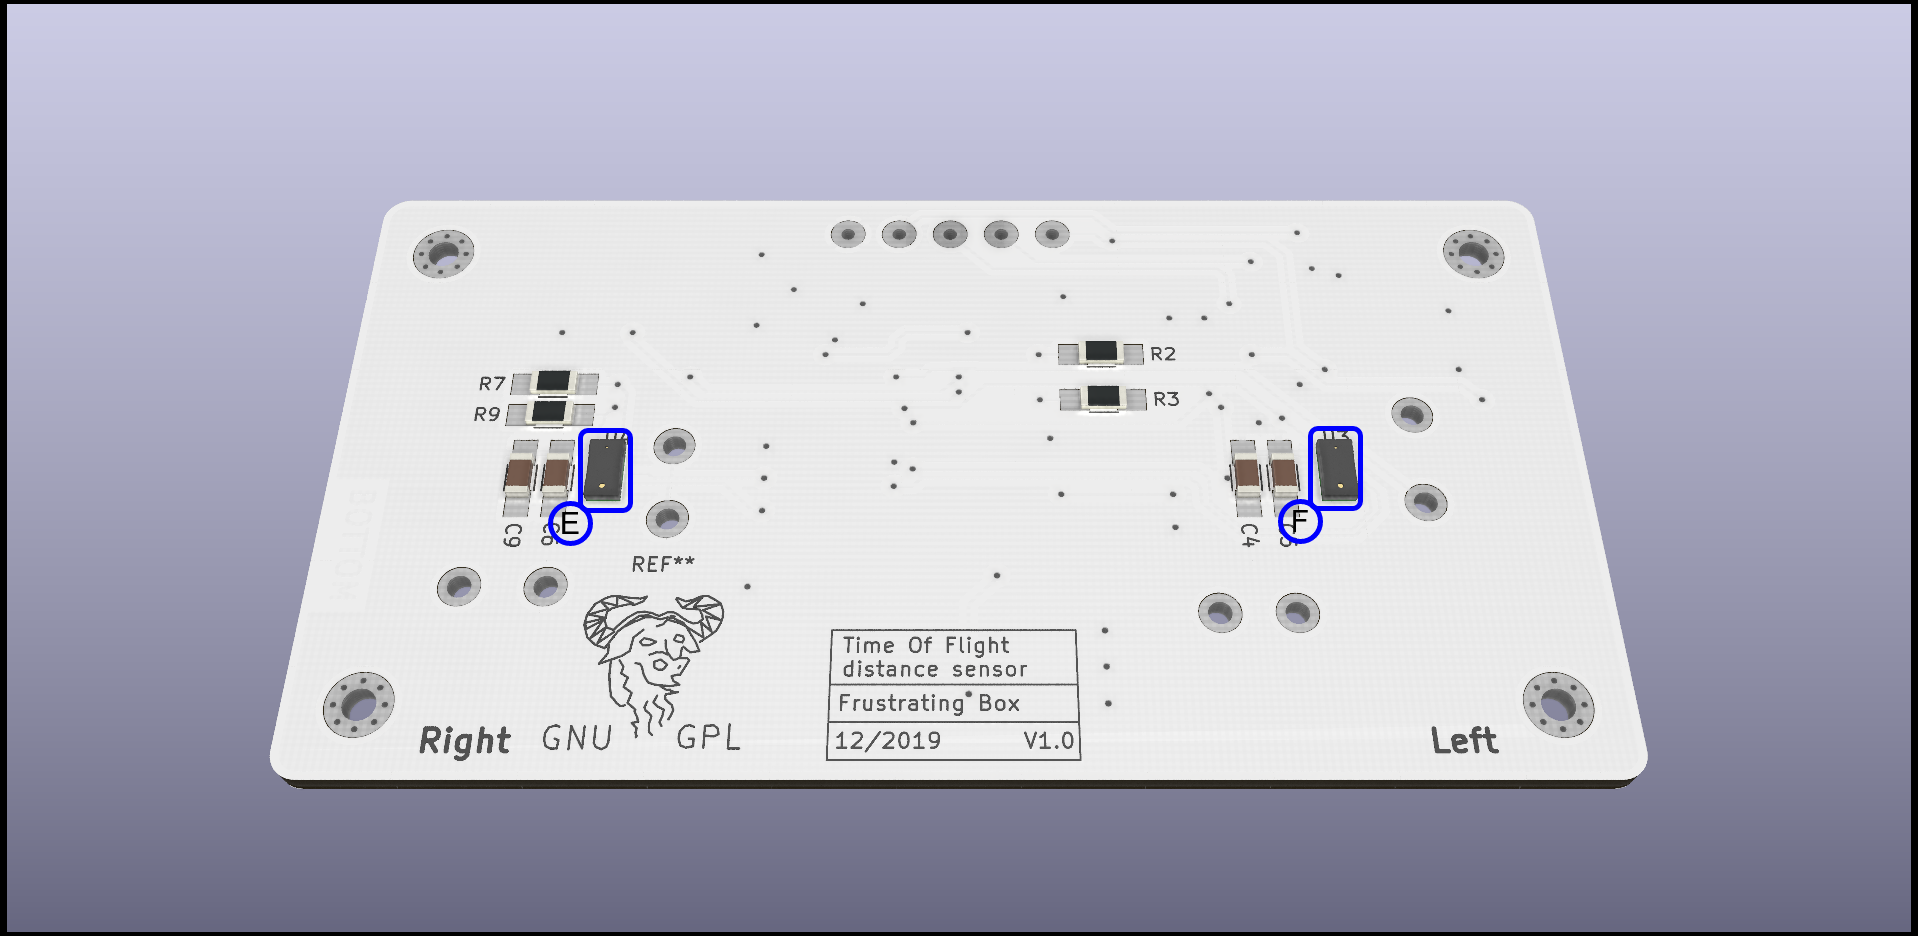
\includegraphics[width=0.75\textwidth]{../img/annotated-layout-back-V1.png}
 \caption{Annotated picture of the back of the sensor}
\end{figure}
\begin{itemize}
 \item[E] Right sensor
 \item[F] Left sensor
\end{itemize}
\pagebreak[4]

\section{Interfacing With the Sensor}
The sensor contains two interfaces. One for using the sensor and one for programming the sensor.
\begin{multicols}{2}
\subsection{Main interface}
The main interface is used for powering the sensor, communication (\iic) and interrupts.
\begin{figure}[H]
 \centering
 
\includegraphics[width=0.2\textwidth]{../img/J2.png}
\end{figure}

\begin{description}
	\item[Power] (Pins \texttt{VCC} and \texttt{GND}) \\
	Sensor can be powered from any source ranging from 3V to 5V connected to \texttt{VCC}. Connect \texttt{GND} to ground. 
	
	\item[\iic] (Pins \texttt{SCL} and \texttt{SDA}) \\
	\iic port. Connect sensor \texttt{SCL} to master \texttt{SCL} and sensor \texttt{SDA} to master \texttt{SDA}.\\
	Compatibility : \cite{i2cspec} \cite{microchipDS}
	\begin{itemize}
		\item standard mode (100kbit/s)
		\item fast mode (400kbit/s)
	\end{itemize}
	
	\item[Interrupts] (Pin \texttt{INT}) \\
	Interrupts output. Pin is driven low when an interrupt is triggered and reset to high when a data register is read.
\end{description}


\columnbreak

\subsection{Programming interface}
\begin{figure}[H]
 \centering
 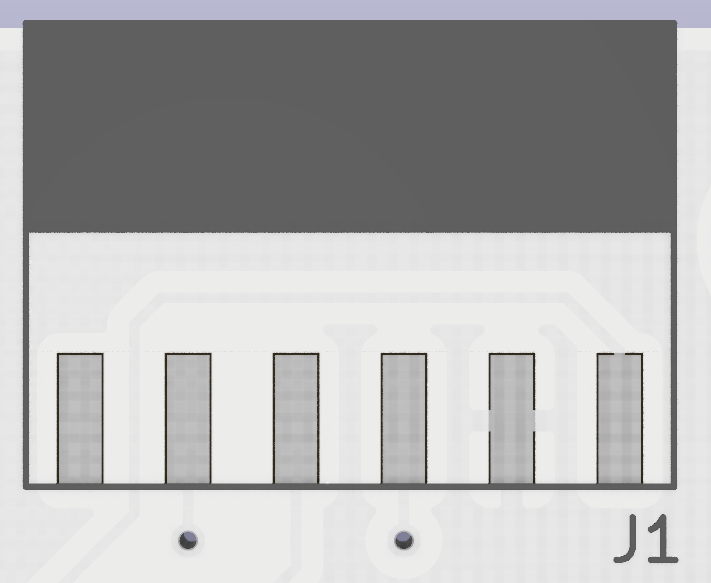
\includegraphics[width=0.2\textwidth]{../img/J1.png}
\end{figure}

	That is the \texttt{ICSP} header used to reprogram the PIC firmware.
	
	\textbf{Note:} On PCB V1.0 the connector is not keyed. VPP is connected to the pin on the right of the picture.
	
	\textbf{Note:} On PCB V1.0 the \texttt{VCC} pin is directly connected to the internal power rail of the sensor. Components on the board are rated to 3.3V and will not tolerate more. Caution must be used when reprogramming the board to not apply more than 3.3V. Advice is to configure the programmer so that it does not power the sensor. Provide 3.0V to 5V yourself via the main interface \texttt{J2}.
	
\end{multicols}
\pagebreak[3]

\section{Registers}
\section{Registers}
Description of the \iic registers.
\subsection{Configuration Registers}
\subsubsection{\texttt{CONFIG\_L}: Configuration register (low part)}
\begin{tabular*}{\textwidth}{@{\extracolsep{\fill}} |c|c|c|c|c|c|c|c|}
 \hline
 \multicolumn{8}{|c|}{\texttt{CONFIG\_L} (0x00)}\\
 \hline
 BIT 7 & BIT 6 & BIT 5 & BIT 4 & BIT 3 & BIT 2 & BIT 1 & BIT 0 \\
 \hline
 \texttt{L\_EN} & \texttt{R\_EN} & \texttt{XTALK} & \texttt{AUTO\_INC} & \texttt{CONT\_MODE} & \texttt{CONV} & \texttt{CONV\_FINISHED} & \texttt{unused}\\
 \hline
\end{tabular*}

\paragraph{} Description of the content of the register:
\begin{description}
 \item[\texttt{L\_EN}] \qquad \textbf{Readable / Writeable / Initialize at 1}\\
       Set this bit to 1 to enable the left sensor.\\
       Set this bit to 0 to disable the left sensor.

 \item[\texttt{R\_EN}] \qquad \textbf{Readable / Writeable / Initialize at 1}\\
       Set this bit to 1 to enable the right sensor.\\
       Set this bit to 0 to disable the right sensor.

 \item[\texttt{XTALK}] \qquad \textbf{Readable / Writeable / Initialize at 0}\\
       Set this bit to 1 to enable crosstalk compensation on both sensors.\\
       Set this bit to 0 to disable crosstalk compensation on both sensors.\\
       More information on crosstalk can be found in the VL53L0X API manual. \cite{tofAPI}

 \item[\texttt{AUTO\_INC}] \qquad \textbf{Readable / Writeable / Initialize at 0}\\
       Set this bit to 1 to enable \iic auto incrementation of the registers.\\
       Set this bit to 0 to disable \iic auto incrementation of the registers.\\
       Auto incrementation of the registers will automatically increment the internal register pointer after a read or a write. The pointer will cycle through the configuration registers if it was initially pointing to a configuration register (and go back to the first config register if it reached the last config register). The pointer will cycle through the data registers if it was initially pointing to a data register (and go back to the first data register if reached the last data register).

 \item[\texttt{CONT\_MODE}] \qquad \textbf{Readable / Writeable / Initialize at 0}\\
       Set this bit to 1 to enable continuous measurement mode.\\
       Set this bit to 0 to disable continuous measurement mode.\\
       Continuous measurement mode will start a new measurement as soon as the last measurement is over. It will also raise the interrupt after each measurement (depending on the interrupt setting) if the interrupt was reset.

 \item[\texttt{CONV}] \qquad \textbf{Readable / Writeable / Hardware clearable / Initialize at 0}\\
       Set this bit to 1 to start a measurement or start continuous measurement.\\
       Set this bit to 0 to stop continuous measurement. If CONT\_MODE is disabled the sensor will automatically clear this bit once the measurement is over.

 \item[\texttt{CONF\_FINISHED}] \qquad \textbf{Read-only / Hardware settable / Hardware clearable / Initialize at 0}\\
       Hardware set to 1 once the conversion is over. \\
       Hardware set to 0 after an \iic read of a data register.
\end{description}

\subsubsection{\texttt{CONFIG\_H}: Configuration register (high part)}\label{reg:configh}
\begin{tabular*}{\textwidth}{@{\extracolsep{\fill}} |c|c|c|c|c|c|c|c|}
 \hline
 \multicolumn{8}{|c|}{\texttt{CONFIG\_H} (0x01)}\\
 \hline
 BIT 7 & BIT 6 & BIT 5 & BIT 4 & BIT 3 & BIT 2 & BIT 1 & BIT 0 \\
 \hline
 \multicolumn{2}{|c|}{\texttt{INT\_MODE}} & \multicolumn{6}{c|}{\texttt{DURATION}}\\
 \hline
\end{tabular*}

\paragraph{} Description of the content of the register:
\begin{description}
 \item[\texttt{INT\_MODE}] \qquad \textbf{Readable / Writeable / Initialize at 0b00}
       \begin{description}
        \item[00] No interrupts. Interrupts are disabled.
        \item[01] Full Interrupt. Generates an interrupt everytime a sensor gets a new measurement.
        \item[10] Half Interrupt. Generates an interrupt once all enabled sensors got a new measurement.\\
              \textit{\textbf{Note :} If only one sensor is enabled the behavior is equivalent to 0b01.}
        \item[11] Unused.
       \end{description}

 \item[\texttt{DURATION}] \qquad \textbf{Readable / Writeable / Initialize at 0b000011}\\
       Controls the time budget allocated to each sensor for it's measurement. The final value is
       $$ \texttt{DURATION}*3 + 20\ [ms]$$
\end{description}

\subsubsection{\texttt{ADDRESS}: \iic Slave Address}
\begin{tabular*}{\textwidth}{@{\extracolsep{\fill}} |c|c|c|c|c|c|c|c|}
 \hline
 \multicolumn{8}{|c|}{\texttt{ADDRESS} (0x02)}\\
 \hline
 BIT 7 & BIT 6 & BIT 5 & BIT 4 & BIT 3 & BIT 2 & BIT 1 & BIT 0 \\
 \hline
 \multicolumn{8}{|c|}{\texttt{ADDRESS}}\\
 \hline
\end{tabular*}

\paragraph{} Description of the content of the register:
\begin{description}
 \item[\texttt{ADDRESS}] \qquad \textbf{Readable / Writeable / Initialize at 0x42}\\
       \iic Address of the device
\end{description}
\textit{\textbf{Note:} If the \iic address of the sensor is changed while in backup address mode the change will only be effective at the next boot in normal \iic address mode.}

\subsection{Data Registers}
All the data registers contains the distance sensed by the two VL53L0X chips. The data are formatted on one byte, unsigned integer representing the distance in centimeters.
All these sensors are read-only.

\begin{description}
 \item[\texttt{Right} (0x10)] Distance measured by the right sensor.
 \item[\texttt{Left} (0x11)] Distance measured by the left sensor.
 \item[\texttt{Min} (0x12)] Minimum distance measured by the sensors.
 \item[\texttt{Max} (0x13)] Maximal distance measured by the sensors.
 \item[\texttt{AVG} (0x14)] Average distance measured by the sensors.
\end{description}

\pagebreak[3]

\section{Boot Configuration and Calibration Routines}
3 boot configuration switches are available on the board to select the boot mode of the sensor.

\subsection{Boot Modes} \label{sec:BootModes}
The first switch controls the main operation mode. Either RUN mode or CAL mode.
\paragraph{In RUN mode} the second switch control the LED behaviour.\\
The third switch control the \iic address.
\paragraph{In CAL mode} the second and third switches control the calibration to perform. The led always displays the status.
\newline
\noindent
\begin{tabularx}{\textwidth}{|c|c|c|X|}
 \hline
 \thead{Switch 1} & \thead{Switch 2} & \thead{Switch 3} & \thead{Behaviour}                                                                                              \\
 \hline
 OFF              & OFF              & OFF              & RUN mode. Status led is always OFF. \iic address is the programmed address (default to 0x42).                  \\
 \hline
 OFF              & OFF              & ON               & RUN mode. Status led is always OFF. \iic address is the backup address (0x44).                                 \\
 \hline
 OFF              & ON               & OFF              & RUN mode. Status led displays status and errors. \iic address is the programmed address (default to 0x42).     \\
 \hline
 OFF              & ON               & ON               & RUN mode. Status led displays status and errors. \iic address is the backup address (0x44).                    \\
 \hline
 ON               & OFF              & OFF              & CAL mode. SPADs calibration routine.                                                                           \\ 
 \hline
 ON               & OFF              & ON               & CAL mode. Offset calibration routine.                                                                          \\
 \hline
 ON               & ON               & OFF              & CAL mode. Crosstalk calibration routine.                                                                       \\
 \hline
 ON               & ON               & ON               & CAL mode. Resets the calibration parameters to the default parameters factory programmed in the VL53L0X chips. \\
 \hline
\end{tabularx}
\textbf{Note:} If you change the \iic address of the sensor while in backup address mode the change will only be effective at the next boot in normal \iic address mode.

\subsection{Calibration routines} %TODO reference to API manual (chap 2)
When booting in calibration mode the status LED will blink a few times (0.5s ON, 0.5s OFF) indicating the calibration routine performed. The LED will then be kept lit until the calibration is over. The LED will then be kept lit off and the sensor can then be safely powered off.

\subsubsection{SPAD Calibration}
Status LED blinks 2 times. Optimize the dynamics of the system. It lasts for approximately 10ms. Nothing special is required to perform this calibration. It must be performed with the protective glass cover if you use one.

\subsubsection{Offset Calibration}
Status LED blinks 3 times. Corrects the mean offset of the measurement compared to the real distance. It lasts for approximately 300ms. To perform this calibration you must place a white target (if possible 88\% reflectance) at precisely 10 cm in front of the sensor in a dark environment. It must be performed with the protective glass cover if you use one.

\subsubsection{Crosstalk Calibration}
Status LED blinks 4 times.
If using a protective window in front of the sensor a sometimes significant fraction of the emitted signal goes back to the sensor after having been reflected by the protective window instead of the target. This leads to false measurements with a non-linear behaviour.
This calibration routine tries to correct those errors and lasts approximately 1sec. To perform this calibration you must place a grey (17\% reflectance) target 50 cm in front of the target. This should be able to correct the crosstalk due to a good quality window. If the window you use produces too much crosstalk this might not suffice to correct the error and you might have to edit the crosstalk calibration parameters in the firmware (\texttt{config.h}).


\subsubsection{Reset}
Status LED blinks 5 times.
All the calibration parameters will be reset to default.
\pagebreak[3]

\section{Error codes}
\section{Error codes}
In RUN mode if the LED is not forced off (see section \ref{sec:BootModes}) the sensor might indicate an error code by blinking the status LED a few times. This should normally not happen during normal operation and is mainly used for debug purposes. The error codes are displayed in table \ref{table:errors}.
\end{multicols}
\noindent
\begingroup
\begin{tabularx}{\textwidth}{|c|X|}
 \hline
 \thead{Number of blinks} & \thead{Reason}                                                                        \\
 \hline
 1                        & Sensor related error during the main execution loop.                                  \\
 \hline
 2                        & Sensor related error while configuring the sensor. (RUN mode only)                    \\
 \hline
 3                        & Could not perform device initialization.                                              \\
 \hline
 4                        & Could not load device specific settings.                                              \\
 \hline
 5                        & \makecell[lc]{In SPAD calibration mode: could not perform SPAD calibration.           \\In reset mod: could not get SPAD calibration data.\\Otherwise: could load SPAD calibration data.}\\
 \hline
 6                        & Could not perform reference calibration.                                              \\
 \hline
 7                        & \makecell[lc]{In offset calibration mode: could not perform offset calibration.       \\In reset mod: could not get offset calibration data.\\Otherwise: could not load offset calibration data.} \\
 \hline
 8                        & \makecell[lc]{In crosstalk calibration mode: could not perform crosstalk calibration. \\In reset mod: could not get crosstalk calibration data.\\Otherwise: could not load crosstalk calibration data.} \\
 \hline
\end{tabularx}
\captionof{table}{List of error codes}\label{table:errors}
\endgroup

\appendix
\newpage
\section{Bill Of Material}
\begin{tabularx}{\textwidth}{|c|c|X|X|}
 \hline
 \thead{Component}               & \thead{Quantity} & \thead{PCB Locations}                  & \thead{Reference used}              \\
 \hline
 PIC24FxxGA702                   & 1                & U2                                     & PIC24FJ256GA702-I/SO                \\
 \hline
 VL53L0X                         & 2                & U3, U4                                 & VL53L0CXV0DH/1                      \\
 \hline
 2.8 LDO Regulator               & 1                & U1                                     & MIC5504-2.8YM5-TR                   \\
 \hline
 \iic Voltage Translator         & 1                & U5                                     & PCA9306DCTR                         \\
 \hline
 ICSP Header [Optional]          & 1                & J1                                     & 10129380-906001ALF                  \\
 \hline
 Canal N Ench. MOSFET            & 1                & Q1                                     & 2N7002K-7                           \\
 \hline
 DIP Switches (3)                & 1                & SW1                                    & 219-3LPS                            \\
 \hline
 Shottky diode                   & 1                & D1                                     & 1PS76SB10,115                       \\
 \hline
 1$\mu$F Capacitor (X5R/X7R)     & 2                & C1, C2                                 & \textit{Any 1206 package capacitor} \\
 \hline
 0.1$\mu$F Capacitor             & 6                & C3, C4, C6, C7, C10, C11               & \textit{Any 1206 package capacitor} \\
 \hline
 4.7$\mu$F Capacitor             & 3                & C5, C8, C9                             & \textit{Any 1206 package capacitor} \\
 \hline
 10$\mu$F Capacitor              & 1                & C12                                    & \textit{Any 1206 package capacitor} \\
 \hline
 \makecell{10k$\Omega$ Resistor} & 9                & R1, R2, R3, R7, R9, R12, R13, R14, R18 & \textit{Any 1206 package resistor}  \\
 \hline
 2.2k$\Omega$ Resistor           & 4                & R4, R5, R6, R8                         & \textit{Any 1206 package resistor}  \\
 \hline
 262.5k$\Omega$ Resistor         & 1                & R10                                    & \textit{Any 1206 package resistor}  \\
 \hline
 200k$\Omega$ Resistor           & 2                & R11, R16                               & \textit{Any 1206 package resistor}  \\
 \hline
 330$\Omega$ Resistor            & 3                & R15, R17, R19                          & \textit{Any 1206 package resistor}  \\
 \hline
 LED                             & 1                & D2                                     & \textit{Any 1206 package LED}       \\
 \hline
\end{tabularx}

\section{Electric Diagram}
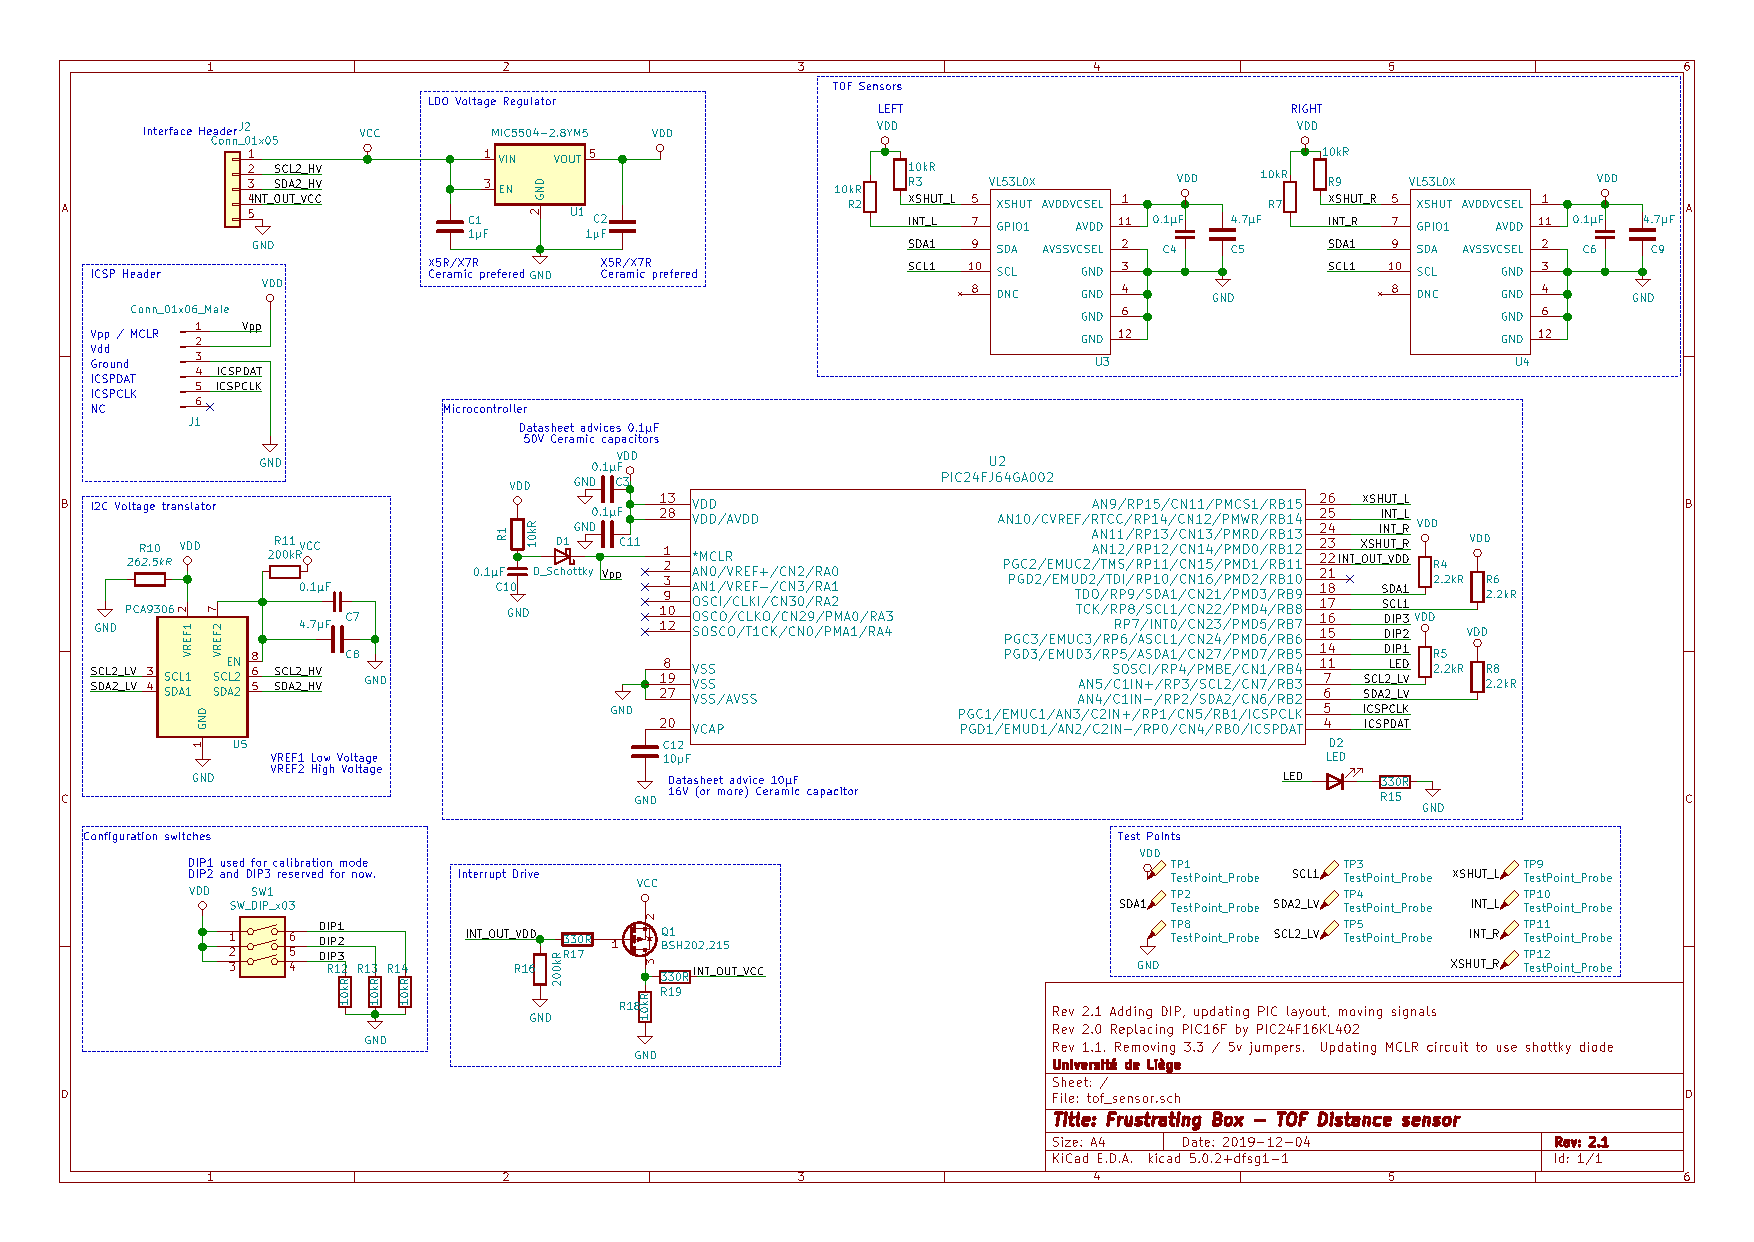
\includepdf[pages=-, landscape]{../documents/schematicV1.pdf}

\nocite{*}
\bibliographystyle{IEEEtran}
\bibliography{main}

\end{document}